\subsubsection{Prerequisites}

If you are intended to use it over Internet, you have to check that there is connectivity between
you and your peers. Parallel Editor uses a port to transmit data. If you are behind a router 
please bear in mind that you will have to forward it.


If you are intended to use it over a LAN, you are ready to go. Usually there are no problems in
using it over a LAN.

For installation instructions see the Installation section. %TODO referenciar a la seccion instalacion

\subsubsection{I have it installed, now what?}

Once you have it installed you're ready to go.

Let's suppose you're working on a Java class (or whatever other language) and you need some help. A 
partner of yours wants to help you with that problem. Both of you are working on the same project, so
both have the project checked out from a SCM in their workstations.

So, you are going to initiate a document editing session. Open up your Java file and right click over it. 
A `Share thru PE' menu should appear right there.

This is how the menu should be seen: 
\begin{figure}[!ht]
	\begin{center}
		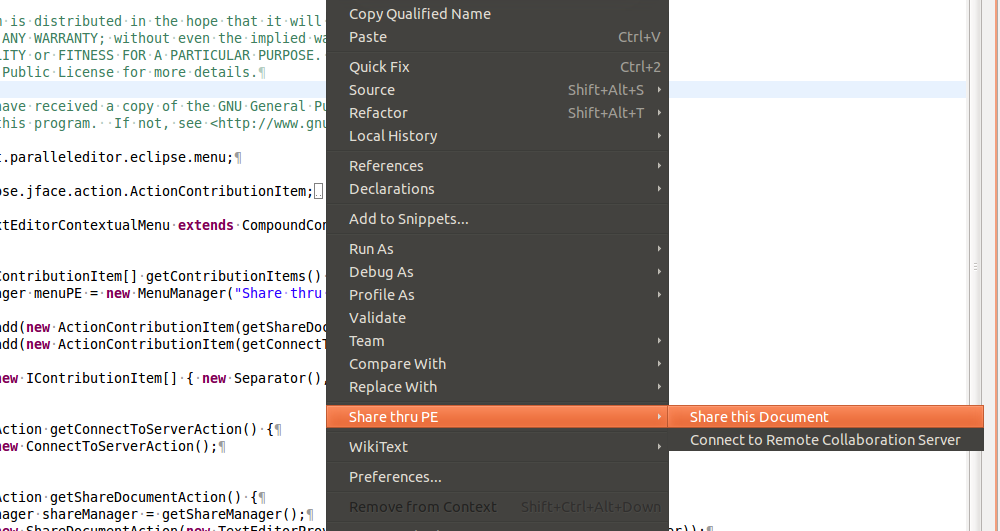
\includegraphics[width=14cm]{contextual_menu.png}
		\caption{\label{share} Share menu.}
	\end{center}
\end{figure}

In this menu, you've got two options. The first one `Share this document' will create a local server 
and share the current file you're editing. After clicking this menu, the Share view will show up.

This view shows all the information you need about your shares and connections. Here we have the screenshot:
\begin{figure}[!ht]
	\begin{center}
		
\includegraphics[width=14cm]{share.png}
		\caption{\label{share} Share views.}
	\end{center}
\end{figure}

You can see the port currently used. In this case, port 5000 is being used. You can give your ip address 
and port to your peers and they can join the session. There is no restriction in how many users can 
edit at the same time.

Also, you can see the users connected to your server and the files being shared.

\subsubsection{Connecting to other sessions}
If a session is already started, you may want to join it. The only thing you need is the ip address and port.
 When you found it out, create a new connection to that server by clicking in `Add hostname' button in the 
 Share view.

When the connection is made, the files shared will appear in the `available documents' section. By 
double-clicking it, you're in.
Every keystroke you make, will be transmited over the network to the peers and they will see the change 
instantly. An optimistic scheme is used, so no lock is acquired over the document.

\subsubsection{Configuration}
Some options are availabe in Eclipse Preferences. You can tweak your default port and default username.
Here we have the screenshot:

\begin{figure}[!ht]
	\begin{center}
		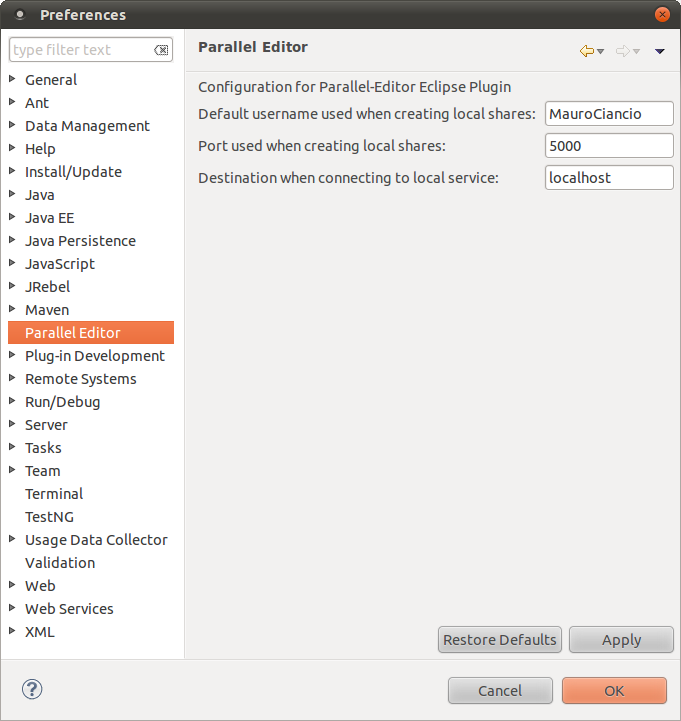
\includegraphics[width=10cm]{preferences.png}
		\caption{\label{preferencias} Preferences dialog}
	\end{center}
\end{figure}

\textbf{Port}: indicates the port on which the local server will listen for remote conections. Make sure
there is no firewall software blocking connections to it.

\textbf{Username}: this is the name that will be used to log on the local server and that your peers will
see when connected to it.

